\newpage 
\ifnum \Version=1
\question[6] Consider the differential equation

$$y'' + 2y' + y = 6e^{-t}, \quad y=y(t)$$    

Solutions to the homogeneous problem are $y_1 = e^{-t}$ and $y_2 = te^{-t}$. 

\begin{parts}
    \part Determine a particular solution to the differential equation using variation of parameters. Do not use undetermined coefficients. \ifnum \Solutions=0 
    \vspace{16cm}
    \fi
    \part State the general solution to the differential equation.
\end{parts}
\ifnum \Solutions=1 {\color{DarkBlue} Solution written below. 
    \begin{figure}[h]
    \centering
    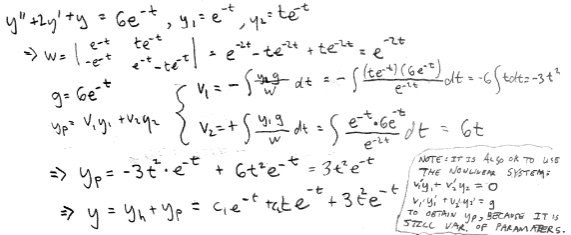
\includegraphics[width=16cm]{Images/ImgTest2VoP.jpg}
    \end{figure}  
} 
\else 
\vspace{3cm}
\fi
\fi


\ifnum \Version=2
\question[6] Consider the differential equation

    $$y'' + p(t)y' + q(t)y = 60t^3, \quad y=y(t)$$    
    
    Solutions to the corresponding homogeneous problem are $y_1 = 1$ and $y_2 = t^2$. 

    \begin{parts}
        \part Determine a particular solution to the differential equation using variation of parameters. Do not use the method of undetermined coefficients. 
        \ifnum \Solutions=0 
        \vspace{16cm}
        \fi
        \part State the general solution to the differential equation.
    \end{parts}
    \ifnum \Solutions=1 {\color{DarkBlue} 
    \begin{enumerate}
    \item[a)] The Wronskian is
\begin{align}
    W = \det \begin{pmatrix} 1&t^2\\0&2t\end{pmatrix} = 2t
\end{align}
To apply the formulas for the variation of parameters method for a second order DE we also use
\begin{align}
    y_1 & = 1 \\
    y_2 &= t^2 \\
    g &= 60t^3 
\end{align}
Applying the formulas for $v_1$ and $v_2$ we obtain
\begin{align}
    v_1 &= - \int \frac{y_2(t)g(t)}{W[y_1,y_2]}dt = - \int \frac{t^2 \cdot 60t^3}{2t} dt = - \int 30 t^4 \, dt = -6t^5 + k_1\\
    v_2 &= \int \frac{y_1(t)g(t)}{W[y_1,y_2]} dt = \int \frac{1\cdot60t^3}{2t} dt = \int 30 t^2 \, dt = 10t^3 + k_2
\end{align}
The arbitrary constants of integration, $k_1$ and $k_2$, in the above are actually not necessary. In the end they will only produce redundant terms because they are solutions to the homogeneous equation. But it is OK to leave them in the expressions for $v_1$ and $v_2$, in the expression for $y_p$, and the expression for $y$. The expression for $y_p$ becomes
\begin{align}
    y_p &= v_1y_1 + v_2y_2 \\
    &= (-6t^5 + k_1)\cdot 1 + (10t^3 + k_2) t^2 \\
    &= -6t^5 + k_1 + 10t^5 + k_2 t^2 \\
    &= 4t^5 + k_1 + k_2t^2
\end{align}
It is OK to ignore the terms with the integration constants and leave the solution as
\begin{align}
    y_p = v_1y_1 + v_2y_2 = -6t^5  + 10t^5 = 4t^5
\end{align}
\item [b)] The general solution to the differential equation is
\begin{align}
    y &= y_h + y_p \\
    &= c_1y_1 + c_2y_2 + v_1y_1 + v_2y_2 \\
    &= c_1 +c_2t^2 + 4t^5 + k_1  + k_2 t^2
\end{align}
Or we can write
\begin{align}
    y &= y_h + y_p  = c_1 +c_2t^2 + 4t^5 
\end{align}
\end{enumerate}
    } 
    \else 
    \fi    
\fi

\ifnum \Version=3
\question[6] Consider the differential equation

    $$y'' + p(t)y' + q(t)y = 60e^{-4t}, \quad y=y(t)$$    
    
    Solutions to the corresponding homogeneous problem are $y_1 = e^t$ and $y_2 = 1$. 
    
    \begin{parts}
        \part Determine a particular solution to the differential equation using variation of parameters. Do not use the method of undetermined coefficients. 
        \ifnum \Solutions=0 
        \vspace{16cm}
        \fi
        \part State the general solution to the differential equation.
    \end{parts}
    \ifnum \Solutions=1 {\color{DarkBlue}  
    \begin{enumerate}
    \item[a)] The Wronskian is
\begin{align}
    W = \det \begin{pmatrix} e^t&1\\e^t&0\end{pmatrix} = -e^t
\end{align}
The formulas for the variation of parameters method for a second order DE also uses:
\begin{align}
    y_1 & = e^t \\
    y_2 &= 1 \\
    g &= 60e^{-4t} 
\end{align}
Applying the formulas for $v_1$ and $v_2$ we obtain
\begin{align}
    v_1 &= - \int \frac{y_2(t)g(t)}{W[y_1,y_2]}dt 
    = - \int \frac{1 \cdot 60e^{-4t}}{-e^t} dt 
    = \int 60e^{-5t} \, dt 
    = -12e^{-5t} + k_1\\
    v_2 &= \int \frac{y_1(t)g(t)}{W[y_1,y_2]} dt 
    = \int \frac{e^t\cdot60e^{-4t}}{-e^t} dt 
    = - \int 60 e^{-4t}\, dt 
    = 15e^{-4t} + k_2
\end{align}
The arbitrary constants of integration, $k_1$ and $k_2$, in the above are actually not necessary. In the end they will only produce redundant terms because they are solutions to the homogeneous equation. But it is OK to leave them in the expressions for $v_1$ and $v_2$, in the expression for $y_p$, and the expression for $y$. 

The expression for $y_p$ becomes
\begin{align}
    y_p &= v_1y_1 + v_2y_2 \\
    &= (-12e^{-5t} + k_1)\cdot e^t + (15e^{-4t} + k_2) \cdot 1 \\
    &= 3e^{-4t} + k_1e^t + k_2
\end{align}
It is OK to ignore the terms with the integration constants and leave the solution as
\begin{align}
    y_p = v_1y_1 + v_2y_2 = 3e^{-4t}
\end{align}
\item [b)] The general solution to the differential equation is
\begin{align}
    y &= y_h + y_p \\
    &= c_1y_1 + c_2y_2 + v_1y_1 + v_2y_2 \\
    &= c_1e^t +c_2 + 3e^{-4t} + k_1e^t + k_2
\end{align}
Or we can write
\begin{align}
    y &= y_h + y_p  = c_1e^t +c_2 + 3e^{-4t} 
\end{align}
\end{enumerate}
    } 
    \else 
    \fi        
\fi


\ifnum \Version=4
\question[6] Consider the differential equation

    $$y'' + p(t)y' + q(t)y = 60t^3, \quad y=y(t)$$    
    
    Solutions to the corresponding homogeneous problem are $y_1 = 1$ and $y_2 = t^2$. 
    
    \begin{parts}
        \part Determine a particular solution to the differential equation using variation of parameters. Do not use the method of undetermined coefficients. 
        \ifnum \Solutions=0 
        \vspace{16cm}
        \fi
        \part State the general solution to the differential equation.
    \end{parts}
    \ifnum \Solutions=1 {\color{DarkBlue}  
    \begin{enumerate}
    \item[a)] The Wronskian is
\begin{align}
    W = \det \begin{pmatrix} 1&t^2\\0&2t\end{pmatrix} = 2t
\end{align}
To apply the formulas for the variation of parameters method for a second order DE we also use
\begin{align}
    y_1 & = 1 \\
    y_2 &= t^2 \\
    g &= 60t^3 
\end{align}
Applying the formulas for $v_1$ and $v_2$ we obtain
\begin{align}
    v_1 &= - \int \frac{y_2(t)g(t)}{W[y_1,y_2]}dt = - \int \frac{t^2 \cdot 60t^3}{2t} dt = - \int 30 t^4 \, dt = -6t^5 + k_1\\
    v_2 &= \int \frac{y_1(t)g(t)}{W[y_1,y_2]} dt = \int \frac{1\cdot60t^3}{2t} dt = \int 30 t^2 \, dt = 10t^3 + k_2
\end{align}
The arbitrary constants of integration, $k_1$ and $k_2$, in the above are actually not necessary. In the end they will only produce redundant terms because they are solutions to the homogeneous equation. But it is OK to leave them in the expressions for $v_1$ and $v_2$, in the expression for $y_p$, and the expression for $y$. The expression for $y_p$ becomes
\begin{align}
    y_p &= v_1y_1 + v_2y_2 \\
    &= (-6t^5 + k_1)\cdot 1 + (10t^3 + k_2) t^2 \\
    &= -6t^5 + k_1 + 10t^5 + k_2 t^2 \\
    &= 4t^5 + k_1 + k_2t^2
\end{align}
It is OK to ignore the terms with the integration constants and leave the solution as
\begin{align}
    y_p = v_1y_1 + v_2y_2 = -6t^5  + 10t^5 = 4t^5
\end{align}
\item [b)] The general solution to the differential equation is
\begin{align}
    y &= y_h + y_p \\
    &= c_1y_1 + c_2y_2 + v_1y_1 + v_2y_2 \\
    &= c_1 +c_2t^2 + 4t^5 + k_1  + k_2 t^2
\end{align}
Or we can write
\begin{align}
    y &= y_h + y_p  = c_1 +c_2t^2 + 4t^5 
\end{align}
\end{enumerate}
    } 
    \else 
    \fi
\fi

\ifnum \Version=5
\question[6] Consider the differential equation

    $$y'' + p(t)y' + q(t)y = 60e^{-4t}, \quad y=y(t)$$    
    
    Solutions to the corresponding homogeneous problem are $y_1 = e^t$ and $y_2 = 1$. 

    \begin{parts}
        \part Determine a particular solution to the differential equation using variation of parameters. Do not use the method of undetermined coefficients. 
        \ifnum \Solutions=0 
        \vspace{16cm}
        \fi
        \part State the general solution to the differential equation.
    \end{parts}
    \ifnum \Solutions=1 {\color{DarkBlue}  
    \begin{enumerate}
    \item[a)] The Wronskian is
\begin{align}
    W = \det \begin{pmatrix} e^t&1\\e^t&0\end{pmatrix} = -e^t
\end{align}
The formulas for the variation of parameters method for a second order DE also uses:
\begin{align}
    y_1 & = e^t \\
    y_2 &= 1 \\
    g &= 60e^{-4t} 
\end{align}
Applying the formulas for $v_1$ and $v_2$ we obtain
\begin{align}
    v_1 &= - \int \frac{y_2(t)g(t)}{W[y_1,y_2]}dt 
    = - \int \frac{1 \cdot 60e^{-4t}}{-e^t} dt 
    = \int 60e^{-5t} \, dt 
    = -12e^{-5t} + k_1\\
    v_2 &= \int \frac{y_1(t)g(t)}{W[y_1,y_2]} dt 
    = \int \frac{e^t\cdot60e^{-4t}}{-e^t} dt 
    = - \int 60 e^{-4t}\, dt 
    = 15e^{-4t} + k_2
\end{align}
The arbitrary constants of integration, $k_1$ and $k_2$, in the above are actually not necessary. In the end they will only produce redundant terms because they are solutions to the homogeneous equation. But it is OK to leave them in the expressions for $v_1$ and $v_2$, in the expression for $y_p$, and the expression for $y$. 

The expression for $y_p$ becomes
\begin{align}
    y_p &= v_1y_1 + v_2y_2 \\
    &= (-12e^{-5t} + k_1)\cdot e^t + (15e^{-4t} + k_2) \cdot 1 \\
    &= 3e^{-4t} + k_1e^t + k_2
\end{align}
It is OK to ignore the terms with the integration constants and leave the solution as
\begin{align}
    y_p = v_1y_1 + v_2y_2 = 3e^{-4t}
\end{align}
\item [b)] The general solution to the differential equation is
\begin{align}
    y &= y_h + y_p \\
    &= c_1y_1 + c_2y_2 + v_1y_1 + v_2y_2 \\
    &= c_1e^t +c_2 + 3e^{-4t} + k_1e^t + k_2
\end{align}
Or we can write
\begin{align}
    y &= y_h + y_p  = c_1e^t +c_2 + 3e^{-4t} 
\end{align}
\end{enumerate}
    } 
    \else 
    \fi    
\fi



\ifnum \Version>5
\question[4] Consider the first order system \[\vec{x} \, ' = \left( \begin{array}{rr} 2 & 4 \\ 4 & 2 \end{array} \right) \vec{x}  + \begin{pmatrix} 24\\0\end{pmatrix}  \]
    
    Solutions to the corresponding homogeneous problem are $\vec x_1 = e^{-2t}\begin{pmatrix} 1\\-1\end{pmatrix}$ and $\vec x_2 = e^{6t}\begin{pmatrix} 1\\1\end{pmatrix}$. 

    \begin{parts}
        \part Determine a particular solution to the differential equation using variation of parameters. Do not use the method of undetermined coefficients. 
\ifnum \Solutions=0 \vspace{17cm}\fi
        \part State the general solution to the system of differential equations. 
    \end{parts}
    \ifnum \Solutions=1 {\color{DarkBlue}   
    
    \begin{itemize}
        \item \textbf{Fundamental Matrix}\\
        The fundamental matrix \(X(t)\) is constructed by placing the solutions \(\vec{x}_1\) and \(\vec{x}_2\) as columns in a matrix. Thus,
        
        \[
        X(t) = \begin{pmatrix} \vec{x}_1 & \vec{x}_2 \end{pmatrix} = \begin{pmatrix} e^{-2t} & e^{6t} \\ -e^{-2t} & e^{6t} \end{pmatrix}
        \]
        \item \textbf{Inverse}\\
        \begin{align*}
            \det(X(t)) &= e^{-2t} \cdot e^{6t} - e^{6t} \cdot (-e^{-2t}) = e^{4t} + e^{4t} = 2e^{4t}\\
            X^{-1} &= \frac{1}{2e^{4t}} \begin{pmatrix} e^{6t} & -e^{6t} \\ e^{-2t} & e^{-2t} \end{pmatrix}
        = \frac{1}{2} \begin{pmatrix} e^{2t} & -e^{2t} \\ e^{-6t} & e^{-6t} \end{pmatrix}
        \end{align*}
        
        \item \textbf{Particular}\\
        \begin{align}
            \vec x_p &= X \int X^{-1} g \, dt \\
            &= X \int \frac{1}{2} \begin{pmatrix} e^{2t} & -e^{2t} \\ e^{-6t} & e^{-6t} \end{pmatrix} \begin{pmatrix} 24 \\ 0 \end{pmatrix} \, dt \\
            & = X \int \begin{pmatrix} 12e^{2t} \\ 12e^{-6t} \end{pmatrix} \, dt \\
            &= \begin{pmatrix} e^{-2t} & e^{6t} \\ -e^{-2t} & e^{6t} \end{pmatrix} \begin{pmatrix} 6e^{2t} + C_1 \\ -2e^{-6t} + C_2 \end{pmatrix} \\
            &=  \begin{pmatrix} 4 + C_1 e^{-2t} + C_2 e^{6t} \\ -8 - C_1 e^{-2t} + C_2 e^{6t} \end{pmatrix}
        \end{align}  
        It is not necessary to keep the $C_1$ and $C_2$ terms, they can be ignored. 
        \item \textbf{General Solution}
        \begin{align}
            \vec x = \vec x_h + \vec x_p = c_1 e^{-2t}\begin{pmatrix} 1\\-1\end{pmatrix} + c_2 e^{6t}\begin{pmatrix} 1\\1\end{pmatrix} + \begin{pmatrix} 4\\-8\end{pmatrix}
        \end{align}

    \end{itemize}




    } 
    \else 
    \fi    
\fi

